\documentclass[paper=a5,pagesize=auto,twoside=false,fontsize=12pt,DIV=classic,BCOR=0mm,headinclude=true,footinclude=false]{scrbook}

%% font selection
\usepackage{utopia}
\usepackage{avant}

%% redefine headers
\usepackage[headsepline]{scrpage2}
\pagestyle{scrheadings}

\setkomafont{author}{%
  \normalfont\normalsize
}

\setkomafont{date}{%
  \normalfont\normalsize
}

\setkomafont{dedication}{%
  \raggedright\normalfont\small\itshape
}

\setkomafont{pageheadfoot}{%
  \normalfont\itshape
}

\automark[chapter]{chapter}
\renewcommand{\chaptermark}[1]{\markboth{#1}{#1}}
%\renewcommand{\sectionmark}[1]{\markright{#1}}

%% additional KOMA script options
\KOMAoptions{parskip=half,headsepline=true,numbers=noendperiod,captions=tableheading}
\recalctypearea{} % recalculate type area after selecting fonts

\usepackage{array}
\usepackage[british]{babel}
\usepackage{bbding}
\usepackage{fancyvrb}
\usepackage{float}  % direct positioning of floats
\usepackage{graphicx}
\usepackage{ifpdf}
\usepackage[utf8x]{inputenc}
\usepackage{paralist}
\usepackage{ucs}
\usepackage[obeyall]{siunitx}
\usepackage[hyphens,obeyspaces]{url}
\usepackage{varioref}
\usepackage{wrapfig}  % must be included after package "float"
\usepackage[dvipsnames]{xcolor}

%% Make sure "hyperref" comes last of your loaded packages, to give it
%% a fighting chance of not being over-written, since its job is to
%% redefine many LATEX commands.
\ifpdf
	\usepackage[unicode,pdftex]{hyperref}
\else
	\usepackage[unicode,hypertex]{hyperref}
\fi

\hypersetup{
  unicode=true,                % non-Latin characters in Acrobat’s bookmarks
  pdftitle=traKmeter,          % title
  pdfauthor=Martin Zuther,     % author
  pdfsubject=traKmeter,        % subject of the document
  pdfcreator=Martin Zuther,    % creator of the document
  colorlinks=true,             % false: boxed links; true: colored links
  linkcolor=blue,              % color of internal links
  citecolor=blue,              % color of links to bibliography
  filecolor=blue,              % color of file links
  urlcolor=blue                % color of external links
}

%% KOMA script captions
\addtokomafont{caption}{\small}
\addtokomafont{captionlabel}{\bfseries}
\setcapindent{0em}

%% taken from package "l2tabu"
\tolerance 1414
\hbadness 1414
\emergencystretch 1.5em
\hfuzz 0.3pt
\widowpenalty=10000
\vfuzz
\hfuzz
\raggedbottom

%% package "fancyvrb"
\DefineVerbatimEnvironment{VerbatimBoth}{Verbatim}{gobble=2,samepage=true,frame=single,framerule=0.4mm,framesep=2mm,xleftmargin=4mm,xrightmargin=4mm,rulecolor=\color{BurntOrange},label=32 and 64 bit}

\DefineVerbatimEnvironment{Verbatim32}{Verbatim}{gobble=2,samepage=true,frame=single,framerule=0.4mm,framesep=2mm,xleftmargin=4mm,xrightmargin=4mm,rulecolor=\color{OrangeRed},label=32 bit}

\DefineVerbatimEnvironment{Verbatim64}{Verbatim}{gobble=2,samepage=true,frame=single,framerule=0.4mm,framesep=2mm,xleftmargin=4mm,xrightmargin=4mm,rulecolor=\color{Cerulean},label=64 bit}

%% package "varioref"
\labelformat{chapter}{chapter~#1}
\labelformat{section}{section~#1}
\labelformat{subsection}{section~#1}
\labelformat{subsubsection}{section~#1}

\labelformat{figure}{figure~#1}
\labelformat{table}{table~#1}

%% package "paralist"
\setdefaultitem{\textbullet}{$\circ$}{}{}

%% package "url"
\urlstyle{rm}

%% package "wrapfig"
\setlength{\intextsep}{0.2\baselineskip}

%% package "siunitx"
\sisetup{per=slash,trapambigfrac,locale=UK}

\newunit[unitspace=space]{\dB}{dB}
\newunit[unitspace=space]{\dBFS}{dB\,FS}
\newunit[unitspace=space]{\dBSPL}{dB\,SPL}
\newunit[unitspace=space]{\dBu}{dBu}
\newunit[unitspace=space]{\LK}{LK}
\newunit[unitspace=space]{\LKFS}{LK\,FS}
\newunit[unitspace=space]{\VRMS}{V\textsubscript{RMS}}
\newunit[unitspace=space]{\VU}{VU}

%% scaling of screenshots
\newcommand{\screenshotscale}{0.7}

%% layout
\usepackage[inner=18mm,outer=18mm,top=26mm,bottom=27mm,headsep=6.5mm,headheight=5mm]{geometry}

% %% start new page for every section
% \let\stdsection\section  
% \renewcommand\section{\newpage\stdsection}

%% command "application"
\DeclareRobustCommand*{\application}[1]{\texttt{#1}}


%%% Local Variables:
%%% mode: latex
%%% mode: outline-minor
%%% TeX-command-default: "Rubber"
%%% TeX-master: "../trakmeter"
%%% TeX-PDF-mode: t
%%% ispell-local-dictionary: "british"
%%% End:

\input{include/hyphenation.sty}

\title{traKmeter}
\author{Martin Zuther}

\begin{document}

\title{traKmeter}

\subtitle{
  \normalsize{\textrm{\textmd{
        \vfill
        Loudness meter for correctly setting up \\
        tracking and mixing levels
        \vfill
        \vspace{1.5em}
        \begin{figure}[H]
          \centering{}
          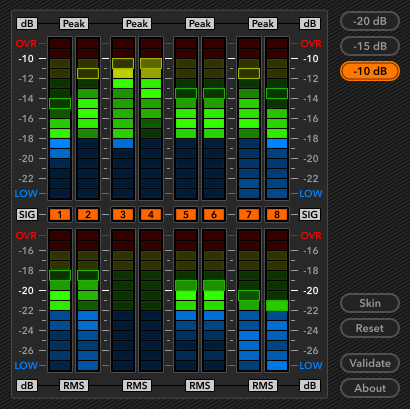
\includegraphics[scale=0.45,clip]{include/images/trakmeter.png}
        \end{figure}
        \vfill
      }}}
}

\author{\normalsize\copyright{} 2012-2013
  \href{http://www.mzuther.de/}{Martin Zuther}}

\date{\normalsize \emph{Last edited on \today}}

\maketitle

\tableofcontents

\clearpage  % layout

\chapter{Digital recordings}
\label{chap:digital_recordings}

The digital revolution brought a lot of advantages to the field of
audio processing such as higher fidelity, less noise and non-degrading
copies.  Unfortunately, however, digital audio also introduced some
problems of its own.

Whereas the analog domain is relatively inert against very high levels
(overdriving some analog equipment actually sounds pretty good), the
digital domain punishes even small transgressions into forbidden
territory with harsh clipping.

And while digital audio can be transferred without loss in quality, it
is degraded by each and every calculation, be it a simple change in
level, equalisation or a fancy effect.  Crossing domains from analog
to digital and \emph{vice versa} leads to additional degradation.
Finally, changes in bit depth and sample rate, jitter and inter-sample
peaks are nothing for the weak of heart.

However, most of these obstacles can be overcome easily by proper gain
staging, minimising the crossing of domains and choosing appropriate
bit depths and sample rates.  If you also learn how to properly test
and operate your equipment, you're well on your way to pure audio
bliss \dots

\section{Gain staging}
\label{sec:gain_staging}

Professional analog audio equipment is designed to be run at a nominal
level of \textbf{\SI[addsign=all]{+4}{\dBu}} (\SI{1.23}{\VRMS}) and
leaves a headroom for peaks of about \SI{20}{\dB}.  This in turn is
consistent with the maximum crest factor of analog audio signals.

Thus, driving all analog audio equipment at \SI[addsign=all]{+4}{\dBu}
ensures an optimal signal-to-noise ratio while preventing clipping and
keeping all transients intact.  The process of setting audio devices
to run at optimal input and output levels is called \emph{gain
  staging}.

Now let's transfer this to the digital domain.  As the maximum crest
factor of analog audio signals amounts to \SI{20}{\dB}, we'll adjust
the headroom accordingly by setting our average input and output
levels to \textbf{\SI{-20}{\dBFS} RMS}.

Again, this ensures a good signal-to-noise ratio while preventing
clipping.  Maybe even more important, this level also drives (most of)
your digital audio equipment and plug-ins at their respective ``sweet
spot''.

Another recommendation is that peak levels should not exceed
\textbf{\SI{-9}{\dBFS}}
(\href{http://tech.ebu.ch/publications/r068}{EBU R68-2000}) during
tracking.  This will leave enough space for sudden jumps in level and
also for inter-sample peaks, audio peaks that lie \emph{in between}
two successive samples and may lead to unpredictable clipping during
digital-to-analog conversion.

Some analog-to-digital converters also degrade audio when fed with
input levels close to digital full-scale (\SI{0}{\dBFS}), resulting in
the ``harshness'' often attributed to digital audio -- my first sound
card certainly suffered from this.  So lowering your input levels as
described above may also improve your overall sound.

Finally, we'll emphasise the newly designated headroom and shift the
meter scales by \SI[addsign=all]{+20}{\dB}.  Thus, the optimal average
audio level is designated \textbf{\SI{0}{\dB} RMS}, while the maximum
peak audio level becomes \textbf{\SI[addsign=all]{+11}{\dB}}.  As a
nice side effect, our new scale corresponds to Bob Katz's
\textbf{\href{http://www.digido.com/level-practices-part-2-includes-the-k-system.html}{K-20
    scale}}.

\section{Digital audio myths}
\label{sec:digital_audio_myths}

I can almost hear you: you have heard that digital recordings should
be performed at peak levels close to but not exceeding \SI{0}{\dBFS}
(digital full-scale).  Heck, this misinformation has ended up in the
manuals of some professional audio equipment.  But for the reasons
given above it is plain wrong.

\begin{wrapfigure}{r}{0pt}
  \includegraphics[scale=0.24,clip]{include/images/level_meter_otari.png}
\end{wrapfigure}

Let's look at a worst-case scenario: even if your recordings
\emph{peak} at \SI{-20}{\dBFS} and you discard the least significant
bit (some people claim that it mostly consists of errors), a bit depth
of 16 bit would still leave you with a signal-to-noise ratio of
\SI{70}{\dB}.  That is about what you can expect from some of the best
professional analog tape machines and recording desks -- and we're not
even talking of 24 bit.

If you don't believe me yet, take a look at my professional 16-bit
hard disk recorder (Otari PD-80): its analog inputs and outputs are
aligned to ``\SI[addsign=all]{+4}{\dBu} (\textbf{\SI{-15}{\dB}} from
digital full-scale)''.  The manufacturer has even marked this level on
the meter bridge (small triangle on the photo).  Although I admit that
the mark is only useful for audio alignment, given that it sits on a
peak meter \dots

There is also a great thread over at Gearslutz (``The Reason Most ITB
mixes don’t Sound as good as Analog mixes'') well worth reading.  Here
are links to the
\href{http://www.gearslutz.com/board/5062929-post1.html}{first post}
and two other selected posts
(\href{http://www.gearslutz.com/board/5064831-post1874.html}{\#1874}
and
\href{http://www.gearslutz.com/board/5609740-post3614.html}{\#3614}).

\section{Introducing traKmeter}
\label{sec:introducing_trakmeter}

Most digital audio equipment sadly only has peak meters.  This is
readily understandable as you want to avoid digital clippings by all
means.  However, the lack of average meters makes correct gain staging
almost impossible.

For gain staging, you need average meters or -- even better -- a
combination of peak and average meters.  And this is were
\textbf{traKmeter} comes in.

\chapter{traKmeter}
\label{chap:trakmeter}

\begin{wrapfigure}{r}{0.18\linewidth}
  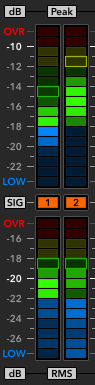
\includegraphics[scale=0.625,clip]{include/images/level_meter_complete.png}
\end{wrapfigure}

\textbf{traKmeter} consists of two meters, a peak meter on top and an
average meter below.  The meters are separated by a blue signal LED
and consist of an area of green LEDs that is enclosed by first yellow
and then red LEDs.

You may have noticed that the average meter's green area is centred
around the \textbf{\SI{0}{\dB} RMS} mark.  This number should be
vaguely familiar.  Remember, it corresponds to \SI{-20}{\dBFS} RMS,
the level we have determined to be the optimal average audio level in
the digital domain.

A fully lit yellow LED on the peak meter's top end corresponds to a
level of \textbf{\SI[addsign=all]{+11}{\dB}} (or \SI{-9}{\dBFS}).
Again, this number should be familiar: peak levels in the digital
domain shouldn't exceed this level.

Thus, by keeping the meter's readout in the green areas and from
entering the yellow and red areas on top of each meter, you will
automatically track at optimal audio levels.

\section{Tracking with traKmeter}
\label{sec:tracking_with_trakmeter}

Open up an instance of \textbf{traKmeter} and set it up so that it
measures your audio input.  That can be done either by starting the
standalone version and connecting it to one or more input channels of
your sound card, or by inserting a plug-in instance into an input
channel of your digital audio workstation.

In the second case, take care that your digital audio workstation
doesn't add additional headroom and that no processing takes place
before \textbf{traKmeter}.  This can be ascertained by feeding
calibration tones into your sound card or by directly comparing the
readouts of standalone and plug-in version.

\begin{wrapfigure}{r}{0.42\linewidth}
  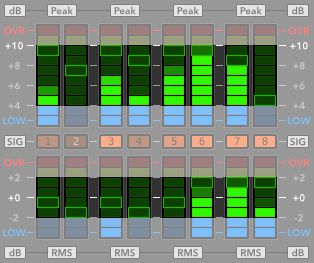
\includegraphics[scale=0.45,clip]{include/images/trakmeter_optimal.png}
\end{wrapfigure}

Now, feed the signal you want to record into an audio input channel
and adjust its level (in the analog domain!) using \textbf{traKmeter}.
Try to set the input level so that transients fall into the average
meter's \textbf{\SI{0}{\dB} RMS} area.  Make sure that peak levels
never exceed \textbf{\SI[addsign=all]{+11}{\dB}}.  In case both
conditions cannot be met simultaneously, adjust the peak level only.
See the image to the right for a visual clue.

\section{Mixing with traKmeter}
\label{sec:mixing_with_trakmeter}

When you get someone else's tracks for mixing, chances are that they
have been recorded far too hot.  While you can't change that, you
might want to adjust them to optimal loudness so that your upcoming
mix is not ruined.

If the original recordings were made with poor equipment and you have
the time, it may be worth to \textbf{re-record} all tracks through a
really good preamp and adjust their loudness at the same time.
Depending on the preamp, the results can be stunning!

Another option is to insert \textbf{traKmeter} on each channel as
first plug-in, enable the ``Mixing'' button (see
\ref{sec:mixing_button}) and adjust volume using the gain knob.

In any case, mixing levels will now be much lower than what you are
used to.  This can easily be corrected by either adjusting the output
gain of your subgroups or by inserting a gain plug-in in your master
track.

To preserve all transients, the final loudness of your mix should stay
within \textbf{\SI{-20}{\dBFS} RMS} and \textbf{\SI{-16}{\dBFS} RMS}
(or between \textbf{\SI{0}{\dB} RMS} and
\textbf{\SI[addsign=all]{+4}{\dB} RMS} on the K-20 scale).  Remember
that smashed transients will be gone forever, whereas you can always
bring up the volume during mastering!  My plug-in
\href{http://code.mzuther.de/}{\textbf{K-Meter}} and its K-20 scale
may help you with setting up correct mixing levels.

\chapter{Installation}
\label{chap:installation}

In order to use the pre-compiled binaries, simply extract the
\textbf{traKmeter} files from the downloaded archive.  For the
plug-ins, you'll then have to move the extracted files to your
respective plug-in folder (\path{~/.lv2}, \path{~/.vst},
\path{C:\Program Files\Steinberg\VstPlugins\} or the like).

\chapter{Controls}
\label{chap:controls}

\section{Reset button}
\label{sec:reset_button}

\begin{wrapfigure}{r}{0.14\linewidth}
  \includegraphics[scale=\screenshotscale,clip]{include/images/button_reset.png}
\end{wrapfigure}

Click on this button to reset all meters.  You can also use it to get
rid of graphical artifacts, because the meters will be redrawn as
well.

\section{Crest factor button}
\label{sec:crest_factor_button}

\begin{wrapfigure}{r}{0.14\linewidth}
  
\includegraphics[scale=\screenshotscale,clip]{include/images/button_crest_factor_on.png}
  \newline \vspace{-0.9\baselineskip}
  
\includegraphics[scale=\screenshotscale,clip]{include/images/button_crest_factor_off.png}
\end{wrapfigure}

When this button is pressed, meter readout uses the K-20 scale (crest
factor of \SI{20}{\dB}).  Disengage the button to change to decibels
relative to digital full-scale (crest factor of \SI{0}{\dB}).

\emph{Please note that although this meter uses the K-20 scale, it is
  by no means a K-System meter.}

\newpage %% layout

\section{Transient button}
\label{sec:transient_button}

\begin{wrapfigure}{r}{0.14\linewidth}
  
\includegraphics[scale=\screenshotscale,clip]{include/images/button_transient_on.png}
  \newline \vspace{-0.9\baselineskip}
  
\includegraphics[scale=\screenshotscale,clip]{include/images/button_transient_off.png}
\end{wrapfigure}

This button changes the RMS meter's ballistics from ``transient'' mode
to ``classic'' mode.

I find that ``transient'' mode with its fast attack and slow release
times is well suited to setting up levels.  It works fine for both
transient audio sources (drums, percussion, piano) and more ``static''
ones (pads, bass and so on).

If you are used to VU meters, however, ``classic'' mode with its
equally slow attack and release times may feel more comfortable to
you.

\emph{\underline{Note:} I don't use ``classic'' mode myself, so you
  may find that the RMS meter scale needs adjusting.  Please don't
  hesitate to notify me, it's really easy to change this.}

\section{Mixing button}
\label{sec:mixing_button}

\begin{wrapfigure}{r}{0.14\linewidth}
  
\includegraphics[scale=\screenshotscale,clip]{include/images/button_mixing_on.png}
  \newline \vspace{-0.9\baselineskip}
  
\includegraphics[scale=\screenshotscale,clip]{include/images/button_mixing_off.png}
\end{wrapfigure}

You can use \textbf{traKmeter} as a gain plug-in -- just enable this
button and adjust the gain knob.

When the plug-in is closed, its meters aren't updated, so it uses less
system resources.  On slow computers, however, use \textbf{traKmeter}
to find the correct gain and then exchange it against a simple gain
plug-in.

Please keep in mind that this setting should only be used for
\textbf{pre-recorded material}.  The gain stage sits \emph{before} the
meter and thus affects the meter's read-out.  So if you apply a
negative gain during recording, your analog input stage might clip
without the meters hitting the red area!

\section{Validation button}
\label{sec:validation_button}

\begin{wrapfigure}{r}{0.14\linewidth}
  
\includegraphics[scale=\screenshotscale,clip]{include/images/button_validate_on.png}
  \newline \vspace{-0.9\baselineskip}
  
\includegraphics[scale=\screenshotscale,clip]{include/images/button_validate_off.png}
\end{wrapfigure}

Click on this button to open the \textbf{validation window} (see
\ref{chap:validation}) which allows you to play an audio file (WAV,
AIFF or FLAC) through \textbf{traKmeter} and dump internal data.
During validation, the button will light up and clicking it will stop
validation early.

\emph{Unfortunately, the underlying JUCE library does not seem to
  support multi-channel audio files.  You may load such audio files
  into your DAW of choice and insert \textbf{traKmeter} as a plug-in
  instance.}

On Linux, dumped data will be written to \path{stderr}, so just start
the \textbf{traKmeter} standalone or your VST host from the shell and
watch the output coming.  On other systems, have a look at your VST
host's log files (I have successfully used Ableton Live for this).  If
that doesn't work, you might have to start either the
\textbf{traKmeter} standalone or your VST host from a debugger.

As a side note, \textbf{SMA(50)} designates the simple moving average
of 50 values, a neat way to emphasise trends and eliminate short-term
fluctuations.

\section{About button}

\begin{wrapfigure}{r}{0.14\linewidth}
  
\includegraphics[scale=\screenshotscale,clip]{include/images/button_about_on.png}
  \newline \vspace{-0.9\baselineskip}
  
\includegraphics[scale=\screenshotscale,clip]{include/images/button_about_off.png}
\end{wrapfigure}

Clicking on this button will open the \textbf{about window} where you
will be informed about version number, contributors, copyright and the
GNU General Public License.

\section{Display license}

\begin{wrapfigure}{r}{0.15\linewidth}
  
\includegraphics[scale=\screenshotscale,clip]{include/images/button_gpl_on.png}
  \newline \vspace{-0.9\baselineskip}
  
\includegraphics[scale=\screenshotscale,clip]{include/images/button_gpl_off.png}
\end{wrapfigure}

This button is located in the \textbf{about window} and does not only
advertise that you are using free software licensed under the
\textbf{GNU General Public License} -- when clicked, it will also open
the license's website in your web browser \dots

\chapter{Meters}
\label{chap:meters}

All meters possess a completely flat frequency response.  Meter scales
can be adjusted using the ``Crest factor'' button (see
\ref{sec:crest_factor_button}).

\section{Average level meter}

\begin{wrapfigure}{r}{0.18\linewidth}
  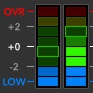
\includegraphics[scale=0.625,clip]{include/images/level_meter_average.png}
\end{wrapfigure}

The average level meter uses an averaging period of \num{1024}
samples.  It has been calibrated according to
\href{http://www.aes.org/publications/standards/search.cfm?docID=21}{AES17-1998}
so that sine wave signals read the same on both peak and average
meters.

Peaks will be held for \SI{10}{\second} and then fall with a speed of
\SI{8.67}{\dB\per\second}.

\subsection{Transient mode}

On rising levels, it takes \SI{10}{\milli\second} for the meter to
reach \SI{99}{\percent} of the final reading.  On falling levels, the
meter switches to a linear fall time of \SI{6}{\dB\per\second}.

\subsection{Classic mode}

Similar to VU meters, it takes \SI{300}{\milli\second} for the meter
to reach \SI{99}{\percent} of the final reading.  This meter exhibits
no overshoot, however.

\section{Peak level meter}

\begin{wrapfigure}{r}{0.18\linewidth}
  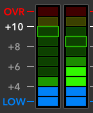
\includegraphics[scale=0.625,clip]{include/images/level_meter_peak.png}
\end{wrapfigure}

The peak level meter has a rise time of one sample and a fall time of
\SI{8.67}{\dB\per\second}.  The red LED marked ``OVR'' detects levels
exceeding \SI{-9}{\dBFS} and should never light.

Peaks will be indefinitely held until the meter is reset.

\section{Signal meter}

\begin{wrapfigure}{r}{0.18\linewidth}
  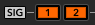
\includegraphics[scale=0.625,clip]{include/images/level_meter_signal.png}
\end{wrapfigure}

The blue signal meter detects peak levels of \SI{-60}{\dBFS} and
above.  It has a rise time of one sample and falls to
\SI{99}{\percent} of the final reading in \SI{1.2}{\second}.

\chapter{Recording tips}
\label{chap:recording_tips}

Over the years, I have accumulated a couple of recording tips.  You
may not know some of them, so read ahead \dots

\begin{description}

\item[Use a good preamp.]  ``Good'' doesn't mean your preamp has to
  have a lot of channels or features.  To the contrary!  Go for a
  simple design and invest your money in professional quality instead.
  Recordings made with a good preamp make mixing much easier -- the
  tracks simply seem to fall into place.

\item[ Use the preamp's gain control.]  If necessary, crank up the
  preamp to yield the needed output level.  Do not fear the preamp's
  internal noise -- making up for low gain in later stages will likely
  result in even more noise!  Also see \ref{sec:gain_staging}.

\item[Avoid unballanced equipment.]  Run all signals on balanced lines
  with a nominal level of \SI[addsign=all]{+4}{\dBu}.  If you can't,
  use DI boxes or transformers and read the previous sentence again
  \dots

\item[Use short audio chains.]  All equipment adds noise or may
  otherwise degrade audio, so keep your audio recording chains as
  short as possible.

  For example, instead of routing your mixer between preamp and hard
  disk recorder, connect the mixer to your hard disk recorder's
  \emph{outputs}.  This simple change can lead to much better
  recordings (especially with cheap mixers) and you'll still be able
  to hear yourself and other tracks during recording.

\item[Record at lower levels.]  Record digital audio at
  \textbf{\SI{-20}{\dBFS} RMS} with peak levels not exceeding
  \textbf{\SI{-9}{\dBFS}}.  For an in-depth explanation, see
  \ref{sec:gain_staging}.

\item[Record in mono.]  Most audio sources do not contain stereo
  information that is useful in a mixing context (notable exceptions
  are audience recordings, string sections and sometimes pianos).  The
  pseudo-stereo effects of some synthesisers may even cause phasing
  issues in the mixing stage.

  Recording these sources in stereo will only waste space on your hard
  disk and make you miserable during mixing.  So why not record them
  in mono in the first place?

\item[Use high bit depths.]  Do yourself a favour and record at bit
  depths of 24 bit instead of 16 bit.  Although most digital audio
  converters only provide 20 bits of \emph{noise-free} audio, the
  additional bits still provide an incredible amount of extra detail
  and you can record at lower levels without losing information.  When
  properly dithered, changing to a lower bit depth even preserves
  quite a bit of that detail.

  Also, if you edit audio files or apply effects, calculation errors
  are inevitable.  At 24 bit, however, most of these artifacts are
  \SI{48}{\dB} lower in level (and thus inaudible) compared to 16 bit
  audio files.

  Your digital audio workstation's bus should use at least 32 bits
  (floating point) to avoid accumulation of the above-mentioned
  artifacts.

\item[Avoid sample rate conversion.]  Sample rate conversion usually
  degrades audio (especially small changes of a few \si{\kilo\hertz}),
  so try to record at the target sample rate.  For instance, tracking
  for a CD release should be carried out at \SI{44.1}{\kilo\hertz}
  instead of \SI{48}{\kilo\hertz}.

  There are of course exceptions to the rule, for instance you may
  prefer to track on a professional DAT machine (\SI{48}{\kilo\hertz})
  when your only other choice is using a consumer audio interface.

  For tracking at higher sample rates, it pays to use exact multiples
  of your target sample rate (such as \SI{88.2}{\kilo\hertz} instead
  of \SI{96}{\kilo\hertz}) if your hardware and software permit.
  Please note that some professionals actually advise against using
  higher sample rates due to the possible build-up of noise beyond
  \SI{20}{\kilo\hertz}.  It is also much more demanding on your
  computer, audio equipment and plug-ins -- and may not be worth the
  hassle.  Try changing from recording at 16 bit to 24 bit first.

  Finally, only use professional software for sample rate conversion.
  This is by no means a trivial task.

\item[Concentrate on recording.]  When tracking, try to not interfere
  with the flow of the session.  This is easily done by keeping
  editing and mixing to the bare minimum.

  For example, I currently track using an old hard disk recorder, as
  digital audio workstations tend to distract me too much.

\item[Avoid copy'n'paste.]  Quite a lot of today's electronic music
  sounds like (and actually is) one short loop that was ``arranged''
  by occasionally muting some of its tracks.  This takes away all the
  small inaccuracies that happen when humans play instruments.  It
  also makes such tracks sound absolutely lifeless.

  So instead of looping a track, record a couple of takes and comp the
  best ones.  You'll be surprised at the difference it makes!

\item[Do not fix things later.]  A bad recording is a bad recording is
  a bad recording.  You can't really ``fix it in the mix''.  So tools
  like Auto-Tune, extreme EQ or the edit button should be seen as a
  last resort.  It's easy to kill all of a track's vibe in the
  process.

  Instead, record a few more takes.  Treat your room (acoustically and
  in terms of positive vibe).  Experiment with microphone placement.
  Try everything you can to help the musicians perform better.  Maybe
  you even have to look for better musicians \dots

\end{description}

\chapter{Validation}
\label{chap:validation}

I have gone to great lengths to ensure that the meters read correctly.
You want to validate for yourself?  Just download and extract the
source code.  The directory \path{validation} contains instructions
and FLAC-compressed wave files.  A word of warning: these audio files
may \textbf{damage your ears} and speakers, so please watch your
monitor levels!

\begin{wrapfigure}{r}{0.33\linewidth}
  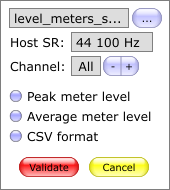
\includegraphics[scale=0.65,clip]{include/images/dialog_validation.png}
\end{wrapfigure}

After opening the \textbf{validation window} (see
\ref{sec:validation_button}), click on the ellipsis button (the one
with the dots) to select an audio file for playback through
\textbf{traKmeter}.  Please make sure that the sample rates of your
host (\textbf{Host SR}) and the audio file match, otherwise the
results will not be correct.

Now, select which \textbf{variables} (if any) should be dumped.  You
may also restrict dumped data to a specific audio \textbf{channel}.
Check \textbf{CSV} if you want to feed the output to a parser.

Finally, click on the \textbf{validate} button to reset all meters and
start playback of the selected audio file.  All audio input will be
discarded during playback and for an additional ten seconds.  To stop
playback early, simply click on the \textbf{validate} button again.

\section{Validation status}

\begin{minipage}{1.0\linewidth}
  \renewcommand{\thempfootnote}{\arabic{mpfootnote}}
  \begin{tabular}{>{\bfseries}llcc}

    &
    \textbf{Test} &
    \textbf{Valid} \\

    Average level meter &
    visuals &
    \Checkmark{} \\

    &
    readout &
    \Checkmark{} \\

    Peak level meter &
    visuals &
    \Checkmark{} \\

    &
    readout &
    \Checkmark{} \\

    Signal meter &
    visuals &
    \Checkmark{} \\

  \end{tabular}
\end{minipage}

\chapter{Help needed}
\label{chap:help_needed}

As \textbf{traKmeter} was coded using cross-platform code, it should
be easy to compile on Mac OS X.  I just don’t have a Mac \dots

In case you want to help, please see the next chapter for an email
address.  You’ll need sufficient experience in coding, compiling and
debugging, though, so no beginners please!

\chapter{Final words}
\label{chap:final_words}

I want to thank \textbf{Rickard} of Interfearing Sounds for asking me
how to use K-Meter for tracking.  This question and the following
thoughts really got \textbf{traKmeter} started.  I'd like to thank
\textbf{bram@smartelectronix} for his code to calculate logarithmic
rise and fall times.  I must also thank the \textbf{beta testers} and
\textbf{users of traKmeter} for sending kind words, suggestions and
bug reports.  Finally, I want to thank the \textbf{open source
  community} for making all of this possible.

Although coding \textbf{traKmeter} has been a lot of fun, it has also
been a lot of work.  So if you like \textbf{traKmeter}, why not send
me a short email and tell me so?  Write a few words about yourself,
send suggestions for future updates or volunteer to create a nice
theme -- do whatever you like!

Here is my email address (please remove ``\texttt{-nospam}''):

\begin{center}
  \texttt{"Martin Zuther" <code-nospam@mzuther.de>}
\end{center}

Thanks for using free software.  I hope you'll enjoy it!

\emph{VST is a trademark of Steinberg Media Technologies GmbH.  ASIO
  is a trademark and software of Steinberg Media Technologies GmbH.}

\appendix

\chapter{How to build traKmeter}
\label{chap:build_trakmeter}

\section{Preparing GNU/Linux}

To build \textbf{traKmeter} yourself, I recommend setting up a
\texttt{chroot} environment.  This is fast and easy to do on
Debian-based systems and might save you a \textbf{lot} of trouble.  At
the time of writing, I'm using Linux Mint 13 (Maya), but the procedure
should be similar on your distribution of choice.  If you aim at
generic \num{64}-bit compilation, simply change \texttt{i386} to
\texttt{amd64}.

To install the necessary packages and install the \texttt{chroot} base
system, execute the following statements (please change
\path{http://ftp.de.debian.org/debian/} to a
\href{http://www.debian.org/mirror/list}{mirror} close to you):

\begin{verbatim}
  sudo apt-get install debootstrap schroot

  sudo mkdir -p /srv/chroot/squeeze_i386
  sudo debootstrap --variant=buildd \
    --arch i386 squeeze \
    /srv/chroot/squeeze_i386 \
    http://ftp.de.debian.org/debian/
\end{verbatim}

Running \path{debootstrap} will take some time.  Meanwhile, add the
following lines to \path{/etc/schroot/schroot.conf} (make sure you
remove all preceding white space so that each line begins in the first
column):

\begin{verbatim}
  [squeeze-i386]
  description=Debian 6 (Squeeze, i386)
  directory=/srv/chroot/squeeze_i386
  personality=linux
  root-users=username
  type=directory
  users=username,another_user
\end{verbatim}

Please make the necessary changes to \texttt{username}.  You may also
add additional users, like \texttt{another\_user}.  In case you are
setting up a \num{32}-bit \texttt{chroot} environment on a
\num{64}-bit system, you'll also have to change \texttt{linux} to
\texttt{linux32}.

When \path{debootstrap} is done, log in as superuser:

\begin{verbatim}
  schroot -c squeeze-i386 -u root
\end{verbatim}

to install a few packages.  The packages \path{less} and \path{vim}
are optional, but might come in handy:

\begin{verbatim}
  apt-get update
  apt-get -y install bash-completion libasound2-dev \
    libjack-jackd2-dev mesa-common-dev xorg-dev
  apt-get -y install less vim
  apt-get clean
\end{verbatim}

If you like \path{bash} completion, you might also want to open the
file \path{/etc/bash.bashrc} and unquote these lines:

\begin{verbatim}
  # enable bash completion in interactive shells
  [two more lines...]
  fi
\end{verbatim}

Finally, log out and log in as normal user:

\begin{verbatim}
  schroot -c squeeze-i386
\end{verbatim}

Congratulations -- after you have installed the dependencies (see
below), you are ready to build \textbf{traKmeter}.

\section{Dependencies}

\subsection{premake4}

\begin{tabbing}
  \hspace*{6em}\=\=\kill

  Importance:  \> required \\
  Version:     \> 4.3 \\
  License:     \> BSD \\
  Homepage:    \> \href{http://industriousone.com/premake}{industriousone.com/premake}
\end{tabbing}

\subsubsection{Installation}

Place the binary somewhere in your \path{PATH}.  Depending on your
platform, you should run \emph{premake} using the scripts
\path{build/run_premake.sh} or \path{build/run_premake.bat}.

\subsection{JUCE library}

\begin{tabbing}
  \hspace*{6em}\=\=\kill

  Importance:  \> required \\
  Version:     \> 2.0.40 \\
  License:     \> GPL v2 \\
  Homepage:    \> \href{http://www.rawmaterialsoftware.com/juce.php}{www.rawmaterialsoftware.com/juce.php}
\end{tabbing}

\subsubsection{Installation}

Extract the archive into the directory \path{libraries/juce}.

\subsection{Virtual Studio Technology SDK}

\begin{tabbing}
  \hspace*{6em}\=\=\kill

  Importance:  \> optional \\
  Version:     \> 2.4 \\
  License:     \> proprietary \\
  Homepage:    \> \href{http://ygrabit.steinberg.de/}{ygrabit.steinberg.de}
\end{tabbing}

\subsubsection{Installation}

Just extract the archive into the directory
\path{libraries/vstsdk2.4}.

\subsection{Audio Streaming Input Output SDK}

\begin{tabbing}
  \hspace*{6em}\=\=\kill

  Importance:  \> optional \\
  Version:     \> 2.2 \\
  License:     \> proprietary \\
  Homepage:    \> \href{http://ygrabit.steinberg.de/}{ygrabit.steinberg.de}
\end{tabbing}

\subsubsection{Installation}

Simply extract the archive into the directory
\path{libraries/asiosdk2.2}.

\subsection{Python}

\begin{tabbing}
  \hspace*{6em}\=\=\kill

  Importance:  \> optional \\
  Version:     \> 3.2 (or higher) \\
  License:     \> Python Software Foundation License \\
  Homepage:    \> \href{http://www.python.org/}{www.python.org}
\end{tabbing}

You'll only need Python if you want to build \num{64}-bit versions of
\textbf{traKmeter} using Visual Studio Express.

\subsubsection{Installation (Windows)}

You can download an installer from the website.  Please also install
the \href{http://msdn.microsoft.com/windows/bb980924.aspx}{Windows
  SDK} and change \path{run_premake.bat} to reflect the SDK's version
number.

\subsection{Artistic Style}

\begin{tabbing}
  \hspace*{6em}\=\=\kill

  Importance:  \> optional \\
  Version:     \> 2.01 \\
  License:     \> LGPL v3 \\
  Homepage:    \> \href{http://astyle.sourceforge.net/}{astyle.sourceforge.net}
\end{tabbing}

This application formats the code so it looks more beautiful and
consistent.  Thus, you only have to install it if you plan to help me
with coding \textbf{traKmeter}.

\subsubsection{Installation}

Place the binary somewhere in your \path{PATH}.  Depending on your
platform, you should run \emph{astyle} using the scripts
\path{src/format_code.sh} or \path{src/format_code.bat}.

\section{Building on GNU/Linux}

After preparing the dependencies, start your \texttt{chroot}
environment, change into the directory \path{build} and execute

\begin{verbatim}
  ./run_premake.sh
  make config=CFG TARGET
\end{verbatim}

where \application{CFG} is one of \application{debug32},
\application{debug64}, \application{release32} and
\application{release64}, and \application{TARGET} is one of
\application{linux\_standalone\_stereo},
\application{linux\_standalone\_multi},
\application{linux\_vst\_stereo} and
\application{linux\_vst\_multi}.

The compiled binaries will end up in the directory \path{bin}.

\section{Building on Microsoft Windows}

After preparing the dependencies, change into the directory
\path{build} and execute

\begin{verbatim}
  ./run_premake.bat
\end{verbatim}

Then change into the directory \path{build/windows/vs20xx}, open the
project file with the corresponding version of Visual C++ and build
the project.

The compiled binaries will end up in the directory \path{bin}.

\section{GNU General Public License}
\label{sec:gpl-3}

\begin{verbatim}

                    GNU GENERAL PUBLIC LICENSE
                       Version 3, 29 June 2007

 Copyright (C) 2007 Free Software Foundation, Inc. <http://fsf.org/>
 Everyone is permitted to copy and distribute verbatim copies
 of this license document, but changing it is not allowed.

                            Preamble

  The GNU General Public License is a free, copyleft license for
software and other kinds of works.

  The licenses for most software and other practical works are designed
to take away your freedom to share and change the works.  By contrast,
the GNU General Public License is intended to guarantee your freedom to
share and change all versions of a program--to make sure it remains free
software for all its users.  We, the Free Software Foundation, use the
GNU General Public License for most of our software; it applies also to
any other work released this way by its authors.  You can apply it to
your programs, too.

  When we speak of free software, we are referring to freedom, not
price.  Our General Public Licenses are designed to make sure that you
have the freedom to distribute copies of free software (and charge for
them if you wish), that you receive source code or can get it if you
want it, that you can change the software or use pieces of it in new
free programs, and that you know you can do these things.

  To protect your rights, we need to prevent others from denying you
these rights or asking you to surrender the rights.  Therefore, you have
certain responsibilities if you distribute copies of the software, or if
you modify it: responsibilities to respect the freedom of others.

  For example, if you distribute copies of such a program, whether
gratis or for a fee, you must pass on to the recipients the same
freedoms that you received.  You must make sure that they, too, receive
or can get the source code.  And you must show them these terms so they
know their rights.

  Developers that use the GNU GPL protect your rights with two steps:
(1) assert copyright on the software, and (2) offer you this License
giving you legal permission to copy, distribute and/or modify it.

  For the developers' and authors' protection, the GPL clearly explains
that there is no warranty for this free software.  For both users' and
authors' sake, the GPL requires that modified versions be marked as
changed, so that their problems will not be attributed erroneously to
authors of previous versions.

  Some devices are designed to deny users access to install or run
modified versions of the software inside them, although the manufacturer
can do so.  This is fundamentally incompatible with the aim of
protecting users' freedom to change the software.  The systematic
pattern of such abuse occurs in the area of products for individuals to
use, which is precisely where it is most unacceptable.  Therefore, we
have designed this version of the GPL to prohibit the practice for those
products.  If such problems arise substantially in other domains, we
stand ready to extend this provision to those domains in future versions
of the GPL, as needed to protect the freedom of users.

  Finally, every program is threatened constantly by software patents.
States should not allow patents to restrict development and use of
software on general-purpose computers, but in those that do, we wish to
avoid the special danger that patents applied to a free program could
make it effectively proprietary.  To prevent this, the GPL assures that
patents cannot be used to render the program non-free.

  The precise terms and conditions for copying, distribution and
modification follow.

                       TERMS AND CONDITIONS

  0. Definitions.

  "This License" refers to version 3 of the GNU General Public License.

  "Copyright" also means copyright-like laws that apply to other kinds of
works, such as semiconductor masks.

  "The Program" refers to any copyrightable work licensed under this
License.  Each licensee is addressed as "you".  "Licensees" and
"recipients" may be individuals or organizations.

  To "modify" a work means to copy from or adapt all or part of the work
in a fashion requiring copyright permission, other than the making of an
exact copy.  The resulting work is called a "modified version" of the
earlier work or a work "based on" the earlier work.

  A "covered work" means either the unmodified Program or a work based
on the Program.

  To "propagate" a work means to do anything with it that, without
permission, would make you directly or secondarily liable for
infringement under applicable copyright law, except executing it on a
computer or modifying a private copy.  Propagation includes copying,
distribution (with or without modification), making available to the
public, and in some countries other activities as well.

  To "convey" a work means any kind of propagation that enables other
parties to make or receive copies.  Mere interaction with a user through
a computer network, with no transfer of a copy, is not conveying.

  An interactive user interface displays "Appropriate Legal Notices"
to the extent that it includes a convenient and prominently visible
feature that (1) displays an appropriate copyright notice, and (2)
tells the user that there is no warranty for the work (except to the
extent that warranties are provided), that licensees may convey the
work under this License, and how to view a copy of this License.  If
the interface presents a list of user commands or options, such as a
menu, a prominent item in the list meets this criterion.

  1. Source Code.

  The "source code" for a work means the preferred form of the work
for making modifications to it.  "Object code" means any non-source
form of a work.

  A "Standard Interface" means an interface that either is an official
standard defined by a recognized standards body, or, in the case of
interfaces specified for a particular programming language, one that
is widely used among developers working in that language.

  The "System Libraries" of an executable work include anything, other
than the work as a whole, that (a) is included in the normal form of
packaging a Major Component, but which is not part of that Major
Component, and (b) serves only to enable use of the work with that
Major Component, or to implement a Standard Interface for which an
implementation is available to the public in source code form.  A
"Major Component", in this context, means a major essential component
(kernel, window system, and so on) of the specific operating system
(if any) on which the executable work runs, or a compiler used to
produce the work, or an object code interpreter used to run it.

  The "Corresponding Source" for a work in object code form means all
the source code needed to generate, install, and (for an executable
work) run the object code and to modify the work, including scripts to
control those activities.  However, it does not include the work's
System Libraries, or general-purpose tools or generally available free
programs which are used unmodified in performing those activities but
which are not part of the work.  For example, Corresponding Source
includes interface definition files associated with source files for
the work, and the source code for shared libraries and dynamically
linked subprograms that the work is specifically designed to require,
such as by intimate data communication or control flow between those
subprograms and other parts of the work.

  The Corresponding Source need not include anything that users
can regenerate automatically from other parts of the Corresponding
Source.

  The Corresponding Source for a work in source code form is that
same work.

  2. Basic Permissions.

  All rights granted under this License are granted for the term of
copyright on the Program, and are irrevocable provided the stated
conditions are met.  This License explicitly affirms your unlimited
permission to run the unmodified Program.  The output from running a
covered work is covered by this License only if the output, given its
content, constitutes a covered work.  This License acknowledges your
rights of fair use or other equivalent, as provided by copyright law.

  You may make, run and propagate covered works that you do not
convey, without conditions so long as your license otherwise remains
in force.  You may convey covered works to others for the sole purpose
of having them make modifications exclusively for you, or provide you
with facilities for running those works, provided that you comply with
the terms of this License in conveying all material for which you do
not control copyright.  Those thus making or running the covered works
for you must do so exclusively on your behalf, under your direction
and control, on terms that prohibit them from making any copies of
your copyrighted material outside their relationship with you.

  Conveying under any other circumstances is permitted solely under
the conditions stated below.  Sublicensing is not allowed; section 10
makes it unnecessary.

  3. Protecting Users' Legal Rights From Anti-Circumvention Law.

  No covered work shall be deemed part of an effective technological
measure under any applicable law fulfilling obligations under article
11 of the WIPO copyright treaty adopted on 20 December 1996, or
similar laws prohibiting or restricting circumvention of such
measures.

  When you convey a covered work, you waive any legal power to forbid
circumvention of technological measures to the extent such circumvention
is effected by exercising rights under this License with respect to
the covered work, and you disclaim any intention to limit operation or
modification of the work as a means of enforcing, against the work's
users, your or third parties' legal rights to forbid circumvention of
technological measures.

  4. Conveying Verbatim Copies.

  You may convey verbatim copies of the Program's source code as you
receive it, in any medium, provided that you conspicuously and
appropriately publish on each copy an appropriate copyright notice;
keep intact all notices stating that this License and any
non-permissive terms added in accord with section 7 apply to the code;
keep intact all notices of the absence of any warranty; and give all
recipients a copy of this License along with the Program.

  You may charge any price or no price for each copy that you convey,
and you may offer support or warranty protection for a fee.

  5. Conveying Modified Source Versions.

  You may convey a work based on the Program, or the modifications to
produce it from the Program, in the form of source code under the
terms of section 4, provided that you also meet all of these conditions:

    a) The work must carry prominent notices stating that you modified
    it, and giving a relevant date.

    b) The work must carry prominent notices stating that it is
    released under this License and any conditions added under section
    7.  This requirement modifies the requirement in section 4 to
    "keep intact all notices".

    c) You must license the entire work, as a whole, under this
    License to anyone who comes into possession of a copy.  This
    License will therefore apply, along with any applicable section 7
    additional terms, to the whole of the work, and all its parts,
    regardless of how they are packaged.  This License gives no
    permission to license the work in any other way, but it does not
    invalidate such permission if you have separately received it.

    d) If the work has interactive user interfaces, each must display
    Appropriate Legal Notices; however, if the Program has interactive
    interfaces that do not display Appropriate Legal Notices, your
    work need not make them do so.

  A compilation of a covered work with other separate and independent
works, which are not by their nature extensions of the covered work,
and which are not combined with it such as to form a larger program,
in or on a volume of a storage or distribution medium, is called an
"aggregate" if the compilation and its resulting copyright are not
used to limit the access or legal rights of the compilation's users
beyond what the individual works permit.  Inclusion of a covered work
in an aggregate does not cause this License to apply to the other
parts of the aggregate.

  6. Conveying Non-Source Forms.

  You may convey a covered work in object code form under the terms
of sections 4 and 5, provided that you also convey the
machine-readable Corresponding Source under the terms of this License,
in one of these ways:

    a) Convey the object code in, or embodied in, a physical product
    (including a physical distribution medium), accompanied by the
    Corresponding Source fixed on a durable physical medium
    customarily used for software interchange.

    b) Convey the object code in, or embodied in, a physical product
    (including a physical distribution medium), accompanied by a
    written offer, valid for at least three years and valid for as
    long as you offer spare parts or customer support for that product
    model, to give anyone who possesses the object code either (1) a
    copy of the Corresponding Source for all the software in the
    product that is covered by this License, on a durable physical
    medium customarily used for software interchange, for a price no
    more than your reasonable cost of physically performing this
    conveying of source, or (2) access to copy the
    Corresponding Source from a network server at no charge.

    c) Convey individual copies of the object code with a copy of the
    written offer to provide the Corresponding Source.  This
    alternative is allowed only occasionally and noncommercially, and
    only if you received the object code with such an offer, in accord
    with subsection 6b.

    d) Convey the object code by offering access from a designated
    place (gratis or for a charge), and offer equivalent access to the
    Corresponding Source in the same way through the same place at no
    further charge.  You need not require recipients to copy the
    Corresponding Source along with the object code.  If the place to
    copy the object code is a network server, the Corresponding Source
    may be on a different server (operated by you or a third party)
    that supports equivalent copying facilities, provided you maintain
    clear directions next to the object code saying where to find the
    Corresponding Source.  Regardless of what server hosts the
    Corresponding Source, you remain obligated to ensure that it is
    available for as long as needed to satisfy these requirements.

    e) Convey the object code using peer-to-peer transmission, provided
    you inform other peers where the object code and Corresponding
    Source of the work are being offered to the general public at no
    charge under subsection 6d.

  A separable portion of the object code, whose source code is excluded
from the Corresponding Source as a System Library, need not be
included in conveying the object code work.

  A "User Product" is either (1) a "consumer product", which means any
tangible personal property which is normally used for personal, family,
or household purposes, or (2) anything designed or sold for incorporation
into a dwelling.  In determining whether a product is a consumer product,
doubtful cases shall be resolved in favor of coverage.  For a particular
product received by a particular user, "normally used" refers to a
typical or common use of that class of product, regardless of the status
of the particular user or of the way in which the particular user
actually uses, or expects or is expected to use, the product.  A product
is a consumer product regardless of whether the product has substantial
commercial, industrial or non-consumer uses, unless such uses represent
the only significant mode of use of the product.

  "Installation Information" for a User Product means any methods,
procedures, authorization keys, or other information required to install
and execute modified versions of a covered work in that User Product from
a modified version of its Corresponding Source.  The information must
suffice to ensure that the continued functioning of the modified object
code is in no case prevented or interfered with solely because
modification has been made.

  If you convey an object code work under this section in, or with, or
specifically for use in, a User Product, and the conveying occurs as
part of a transaction in which the right of possession and use of the
User Product is transferred to the recipient in perpetuity or for a
fixed term (regardless of how the transaction is characterized), the
Corresponding Source conveyed under this section must be accompanied
by the Installation Information.  But this requirement does not apply
if neither you nor any third party retains the ability to install
modified object code on the User Product (for example, the work has
been installed in ROM).

  The requirement to provide Installation Information does not include a
requirement to continue to provide support service, warranty, or updates
for a work that has been modified or installed by the recipient, or for
the User Product in which it has been modified or installed.  Access to a
network may be denied when the modification itself materially and
adversely affects the operation of the network or violates the rules and
protocols for communication across the network.

  Corresponding Source conveyed, and Installation Information provided,
in accord with this section must be in a format that is publicly
documented (and with an implementation available to the public in
source code form), and must require no special password or key for
unpacking, reading or copying.

  7. Additional Terms.

  "Additional permissions" are terms that supplement the terms of this
License by making exceptions from one or more of its conditions.
Additional permissions that are applicable to the entire Program shall
be treated as though they were included in this License, to the extent
that they are valid under applicable law.  If additional permissions
apply only to part of the Program, that part may be used separately
under those permissions, but the entire Program remains governed by
this License without regard to the additional permissions.

  When you convey a copy of a covered work, you may at your option
remove any additional permissions from that copy, or from any part of
it.  (Additional permissions may be written to require their own
removal in certain cases when you modify the work.)  You may place
additional permissions on material, added by you to a covered work,
for which you have or can give appropriate copyright permission.

  Notwithstanding any other provision of this License, for material you
add to a covered work, you may (if authorized by the copyright holders of
that material) supplement the terms of this License with terms:

    a) Disclaiming warranty or limiting liability differently from the
    terms of sections 15 and 16 of this License; or

    b) Requiring preservation of specified reasonable legal notices or
    author attributions in that material or in the Appropriate Legal
    Notices displayed by works containing it; or

    c) Prohibiting misrepresentation of the origin of that material, or
    requiring that modified versions of such material be marked in
    reasonable ways as different from the original version; or

    d) Limiting the use for publicity purposes of names of licensors or
    authors of the material; or

    e) Declining to grant rights under trademark law for use of some
    trade names, trademarks, or service marks; or

    f) Requiring indemnification of licensors and authors of that
    material by anyone who conveys the material (or modified versions of
    it) with contractual assumptions of liability to the recipient, for
    any liability that these contractual assumptions directly impose on
    those licensors and authors.

  All other non-permissive additional terms are considered "further
restrictions" within the meaning of section 10.  If the Program as you
received it, or any part of it, contains a notice stating that it is
governed by this License along with a term that is a further
restriction, you may remove that term.  If a license document contains
a further restriction but permits relicensing or conveying under this
License, you may add to a covered work material governed by the terms
of that license document, provided that the further restriction does
not survive such relicensing or conveying.

  If you add terms to a covered work in accord with this section, you
must place, in the relevant source files, a statement of the
additional terms that apply to those files, or a notice indicating
where to find the applicable terms.

  Additional terms, permissive or non-permissive, may be stated in the
form of a separately written license, or stated as exceptions;
the above requirements apply either way.

  8. Termination.

  You may not propagate or modify a covered work except as expressly
provided under this License.  Any attempt otherwise to propagate or
modify it is void, and will automatically terminate your rights under
this License (including any patent licenses granted under the third
paragraph of section 11).

  However, if you cease all violation of this License, then your
license from a particular copyright holder is reinstated (a)
provisionally, unless and until the copyright holder explicitly and
finally terminates your license, and (b) permanently, if the copyright
holder fails to notify you of the violation by some reasonable means
prior to 60 days after the cessation.

  Moreover, your license from a particular copyright holder is
reinstated permanently if the copyright holder notifies you of the
violation by some reasonable means, this is the first time you have
received notice of violation of this License (for any work) from that
copyright holder, and you cure the violation prior to 30 days after
your receipt of the notice.

  Termination of your rights under this section does not terminate the
licenses of parties who have received copies or rights from you under
this License.  If your rights have been terminated and not permanently
reinstated, you do not qualify to receive new licenses for the same
material under section 10.

  9. Acceptance Not Required for Having Copies.

  You are not required to accept this License in order to receive or
run a copy of the Program.  Ancillary propagation of a covered work
occurring solely as a consequence of using peer-to-peer transmission
to receive a copy likewise does not require acceptance.  However,
nothing other than this License grants you permission to propagate or
modify any covered work.  These actions infringe copyright if you do
not accept this License.  Therefore, by modifying or propagating a
covered work, you indicate your acceptance of this License to do so.

  10. Automatic Licensing of Downstream Recipients.

  Each time you convey a covered work, the recipient automatically
receives a license from the original licensors, to run, modify and
propagate that work, subject to this License.  You are not responsible
for enforcing compliance by third parties with this License.

  An "entity transaction" is a transaction transferring control of an
organization, or substantially all assets of one, or subdividing an
organization, or merging organizations.  If propagation of a covered
work results from an entity transaction, each party to that
transaction who receives a copy of the work also receives whatever
licenses to the work the party's predecessor in interest had or could
give under the previous paragraph, plus a right to possession of the
Corresponding Source of the work from the predecessor in interest, if
the predecessor has it or can get it with reasonable efforts.

  You may not impose any further restrictions on the exercise of the
rights granted or affirmed under this License.  For example, you may
not impose a license fee, royalty, or other charge for exercise of
rights granted under this License, and you may not initiate litigation
(including a cross-claim or counterclaim in a lawsuit) alleging that
any patent claim is infringed by making, using, selling, offering for
sale, or importing the Program or any portion of it.

  11. Patents.

  A "contributor" is a copyright holder who authorizes use under this
License of the Program or a work on which the Program is based.  The
work thus licensed is called the contributor's "contributor version".

  A contributor's "essential patent claims" are all patent claims
owned or controlled by the contributor, whether already acquired or
hereafter acquired, that would be infringed by some manner, permitted
by this License, of making, using, or selling its contributor version,
but do not include claims that would be infringed only as a
consequence of further modification of the contributor version.  For
purposes of this definition, "control" includes the right to grant
patent sublicenses in a manner consistent with the requirements of
this License.

  Each contributor grants you a non-exclusive, worldwide, royalty-free
patent license under the contributor's essential patent claims, to
make, use, sell, offer for sale, import and otherwise run, modify and
propagate the contents of its contributor version.

  In the following three paragraphs, a "patent license" is any express
agreement or commitment, however denominated, not to enforce a patent
(such as an express permission to practice a patent or covenant not to
sue for patent infringement).  To "grant" such a patent license to a
party means to make such an agreement or commitment not to enforce a
patent against the party.

  If you convey a covered work, knowingly relying on a patent license,
and the Corresponding Source of the work is not available for anyone
to copy, free of charge and under the terms of this License, through a
publicly available network server or other readily accessible means,
then you must either (1) cause the Corresponding Source to be so
available, or (2) arrange to deprive yourself of the benefit of the
patent license for this particular work, or (3) arrange, in a manner
consistent with the requirements of this License, to extend the patent
license to downstream recipients.  "Knowingly relying" means you have
actual knowledge that, but for the patent license, your conveying the
covered work in a country, or your recipient's use of the covered work
in a country, would infringe one or more identifiable patents in that
country that you have reason to believe are valid.

  If, pursuant to or in connection with a single transaction or
arrangement, you convey, or propagate by procuring conveyance of, a
covered work, and grant a patent license to some of the parties
receiving the covered work authorizing them to use, propagate, modify
or convey a specific copy of the covered work, then the patent license
you grant is automatically extended to all recipients of the covered
work and works based on it.

  A patent license is "discriminatory" if it does not include within
the scope of its coverage, prohibits the exercise of, or is
conditioned on the non-exercise of one or more of the rights that are
specifically granted under this License.  You may not convey a covered
work if you are a party to an arrangement with a third party that is
in the business of distributing software, under which you make payment
to the third party based on the extent of your activity of conveying
the work, and under which the third party grants, to any of the
parties who would receive the covered work from you, a discriminatory
patent license (a) in connection with copies of the covered work
conveyed by you (or copies made from those copies), or (b) primarily
for and in connection with specific products or compilations that
contain the covered work, unless you entered into that arrangement,
or that patent license was granted, prior to 28 March 2007.

  Nothing in this License shall be construed as excluding or limiting
any implied license or other defenses to infringement that may
otherwise be available to you under applicable patent law.

  12. No Surrender of Others' Freedom.

  If conditions are imposed on you (whether by court order, agreement or
otherwise) that contradict the conditions of this License, they do not
excuse you from the conditions of this License.  If you cannot convey a
covered work so as to satisfy simultaneously your obligations under this
License and any other pertinent obligations, then as a consequence you may
not convey it at all.  For example, if you agree to terms that obligate you
to collect a royalty for further conveying from those to whom you convey
the Program, the only way you could satisfy both those terms and this
License would be to refrain entirely from conveying the Program.

  13. Use with the GNU Affero General Public License.

  Notwithstanding any other provision of this License, you have
permission to link or combine any covered work with a work licensed
under version 3 of the GNU Affero General Public License into a single
combined work, and to convey the resulting work.  The terms of this
License will continue to apply to the part which is the covered work,
but the special requirements of the GNU Affero General Public License,
section 13, concerning interaction through a network will apply to the
combination as such.

  14. Revised Versions of this License.

  The Free Software Foundation may publish revised and/or new versions of
the GNU General Public License from time to time.  Such new versions will
be similar in spirit to the present version, but may differ in detail to
address new problems or concerns.

  Each version is given a distinguishing version number.  If the
Program specifies that a certain numbered version of the GNU General
Public License "or any later version" applies to it, you have the
option of following the terms and conditions either of that numbered
version or of any later version published by the Free Software
Foundation.  If the Program does not specify a version number of the
GNU General Public License, you may choose any version ever published
by the Free Software Foundation.

  If the Program specifies that a proxy can decide which future
versions of the GNU General Public License can be used, that proxy's
public statement of acceptance of a version permanently authorizes you
to choose that version for the Program.

  Later license versions may give you additional or different
permissions.  However, no additional obligations are imposed on any
author or copyright holder as a result of your choosing to follow a
later version.

  15. Disclaimer of Warranty.

  THERE IS NO WARRANTY FOR THE PROGRAM, TO THE EXTENT PERMITTED BY
APPLICABLE LAW.  EXCEPT WHEN OTHERWISE STATED IN WRITING THE COPYRIGHT
HOLDERS AND/OR OTHER PARTIES PROVIDE THE PROGRAM "AS IS" WITHOUT WARRANTY
OF ANY KIND, EITHER EXPRESSED OR IMPLIED, INCLUDING, BUT NOT LIMITED TO,
THE IMPLIED WARRANTIES OF MERCHANTABILITY AND FITNESS FOR A PARTICULAR
PURPOSE.  THE ENTIRE RISK AS TO THE QUALITY AND PERFORMANCE OF THE PROGRAM
IS WITH YOU.  SHOULD THE PROGRAM PROVE DEFECTIVE, YOU ASSUME THE COST OF
ALL NECESSARY SERVICING, REPAIR OR CORRECTION.

  16. Limitation of Liability.

  IN NO EVENT UNLESS REQUIRED BY APPLICABLE LAW OR AGREED TO IN WRITING
WILL ANY COPYRIGHT HOLDER, OR ANY OTHER PARTY WHO MODIFIES AND/OR CONVEYS
THE PROGRAM AS PERMITTED ABOVE, BE LIABLE TO YOU FOR DAMAGES, INCLUDING ANY
GENERAL, SPECIAL, INCIDENTAL OR CONSEQUENTIAL DAMAGES ARISING OUT OF THE
USE OR INABILITY TO USE THE PROGRAM (INCLUDING BUT NOT LIMITED TO LOSS OF
DATA OR DATA BEING RENDERED INACCURATE OR LOSSES SUSTAINED BY YOU OR THIRD
PARTIES OR A FAILURE OF THE PROGRAM TO OPERATE WITH ANY OTHER PROGRAMS),
EVEN IF SUCH HOLDER OR OTHER PARTY HAS BEEN ADVISED OF THE POSSIBILITY OF
SUCH DAMAGES.

  17. Interpretation of Sections 15 and 16.

  If the disclaimer of warranty and limitation of liability provided
above cannot be given local legal effect according to their terms,
reviewing courts shall apply local law that most closely approximates
an absolute waiver of all civil liability in connection with the
Program, unless a warranty or assumption of liability accompanies a
copy of the Program in return for a fee.

                     END OF TERMS AND CONDITIONS

            How to Apply These Terms to Your New Programs

  If you develop a new program, and you want it to be of the greatest
possible use to the public, the best way to achieve this is to make it
free software which everyone can redistribute and change under these terms.

  To do so, attach the following notices to the program.  It is safest
to attach them to the start of each source file to most effectively
state the exclusion of warranty; and each file should have at least
the "copyright" line and a pointer to where the full notice is found.

    <one line to give the program's name and a brief idea of what it does.>
    Copyright (C) <year>  <name of author>

    This program is free software: you can redistribute it and/or modify
    it under the terms of the GNU General Public License as published by
    the Free Software Foundation, either version 3 of the License, or
    (at your option) any later version.

    This program is distributed in the hope that it will be useful,
    but WITHOUT ANY WARRANTY; without even the implied warranty of
    MERCHANTABILITY or FITNESS FOR A PARTICULAR PURPOSE.  See the
    GNU General Public License for more details.

    You should have received a copy of the GNU General Public License
    along with this program.  If not, see <http://www.gnu.org/licenses/>.

Also add information on how to contact you by electronic and paper mail.

  If the program does terminal interaction, make it output a short
notice like this when it starts in an interactive mode:

    <program>  Copyright (C) <year>  <name of author>
    This program comes with ABSOLUTELY NO WARRANTY; for details type `show w'.
    This is free software, and you are welcome to redistribute it
    under certain conditions; type `show c' for details.

The hypothetical commands `show w' and `show c' should show the appropriate
parts of the General Public License.  Of course, your program's commands
might be different; for a GUI interface, you would use an "about box".

  You should also get your employer (if you work as a programmer) or school,
if any, to sign a "copyright disclaimer" for the program, if necessary.
For more information on this, and how to apply and follow the GNU GPL, see
<http://www.gnu.org/licenses/>.

  The GNU General Public License does not permit incorporating your program
into proprietary programs.  If your program is a subroutine library, you
may consider it more useful to permit linking proprietary applications with
the library.  If this is what you want to do, use the GNU Lesser General
Public License instead of this License.  But first, please read
<http://www.gnu.org/philosophy/why-not-lgpl.html>.

\end{verbatim}


\end{document}


%%% Local Variables:
%%% mode: latex
%%% mode: outline-minor
%%% TeX-command-default: "Rubber"
%%% TeX-PDF-mode: t
%%% ispell-local-dictionary: "british"
%%% End:
